\section*{Executive Summary}

\textbf{MediQuiz} is an Intelligent Tutoring System (ITS) engineered for medical students,
addressing two fundamental challenges in medical education:

\begin{itemize}
    \item \textbf{Content Scalability \& Precision:} Transforming dense, 1{,}000-page medical
          textbooks (\textit{Ganong's Medical Physiology}, \textit{Harper's Illustrated Biochemistry},
          \textit{Junqueira's Basic Histology}) into clinically rigorous, verified multiple-choice
          questions (MCQs) and flashcards --- without hallucination.
    \item \textbf{Adaptive Personalization:} Accurately inferring student knowledge states across
          a granular medical taxonomy in real time, delivering customised quizzes, spaced-repetition
          schedules, and intelligent dashboard recommendations.
\end{itemize}

The diagram below illustrates the three decoupled subsystems that compose the full MediQuiz
platform.

\begin{figure}[htbp]
    \centering
    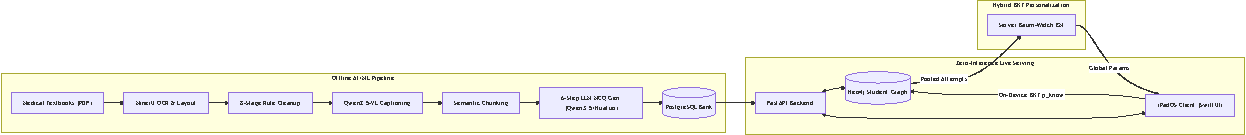
\includegraphics[width=\linewidth]{images/mermaid_exec_summary.pdf}
    \caption{High-level overview of the three MediQuiz subsystems: Offline AI/ML Pipeline,
             Zero-Inference Live Serving, and Hybrid BKT Personalization.}
\end{figure}
